\documentclass[border=7pt]{standalone}
\usepackage{tikz}
\begin{document}
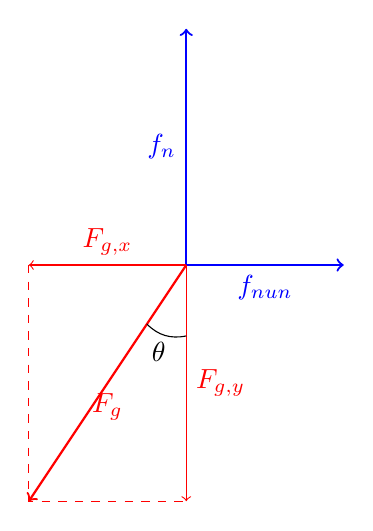
\begin{tikzpicture}
\draw [->, blue, thick](0,0) -- (2,0) node [midway, below]{$f_{nun}$};
\draw [->, blue, thick](0,0) -- (0,3) node [midway, left]{$f_{n}$};
\draw [->, red](0,0) -- (-2,0) node [midway, above]{$F_{g,x}$};
\draw [->, red](0,0) -- (0,-3) node [midway, right]{$F_{g,y}$};
\draw [->, red, thick](0,0) -- (-2,-3) node [midway, below]{$F_{g}$};

\draw [dashed, red] (-2,0) -- (-2,-3) -- (0,-3) ;
\draw (-0.5,-0.75) to [out=-45, in=191.4] (0,-0.901);

\node (c) at (-0.35, -1.1) {$\theta$};


\end{tikzpicture}
\end{document}
